\documentclass[10pt]{article}
\usepackage{fullpage}
\usepackage{graphicx}
\usepackage{float}
\usepackage{amsmath, amsfonts}
\usepackage[utf8]{inputenc}
\usepackage{parskip}

\usepackage{listings}
\usepackage{color}

%New colors defined below
\definecolor{codegreen}{rgb}{0,0.6,0}
\definecolor{codegray}{rgb}{0.5,0.5,0.5}
\definecolor{codepurple}{rgb}{0.58,0,0.82}
\definecolor{backcolour}{rgb}{0.95,0.95,0.92}

%Code listing style named "mystyle"
\lstdefinestyle{mystyle}{
  backgroundcolor=\color{backcolour},   commentstyle=\color{codegreen},
  keywordstyle=\color{magenta},
  numberstyle=\tiny\color{codegray},
  stringstyle=\color{codepurple},
  basicstyle=\footnotesize,
  breakatwhitespace=false,         
  breaklines=true,                 
  captionpos=b,                    
  keepspaces=true,                 
  numbers=left,                    
  numbersep=5pt,                  
  showspaces=false,                
  showstringspaces=false,
  showtabs=false,                  
  tabsize=2
}


\begin{document}
\begin{center}
{{\Large \sc Algorithms and Data Structures 02105+02326}}
\end{center}
\rule{\textwidth}{1pt}
\begin{description}
\item[Student name and id:] Roar Nind Steffensen (s144107)
\item[Teaching assistant:] Martin Hemmingsen
\item[Hand-in for week:] 7
\end{description}

\section*{Exercise M1}
The social network can be depicted at a graph, by mapping all persons $P$ to nodes, and friendship relations $V$ as edges. Since a friendship relation has no direction, meaning that $p_i$ cannot be friends with $p_j$ without $p_j$ being friends with $p_i$ for $p_i$, $p_j \in P$, the simplest graph we can choose, is a non-directed graph. 

\section*{Exercise M2}

The example given has the following persons:
\begin{center}
\{Hans, Børge, Otto, Knud, Finn\}
\end{center}
and friendship relations: 
\begin{center}
\{(Hans, Børge), (Otto, Knud), (Børge, Otto), (Hans, Otto), (Finn, Knud)\}
\end{center}


The graph for this social network is seen on figure \ref{fig:example}

\begin{figure}[H]
    \centering
    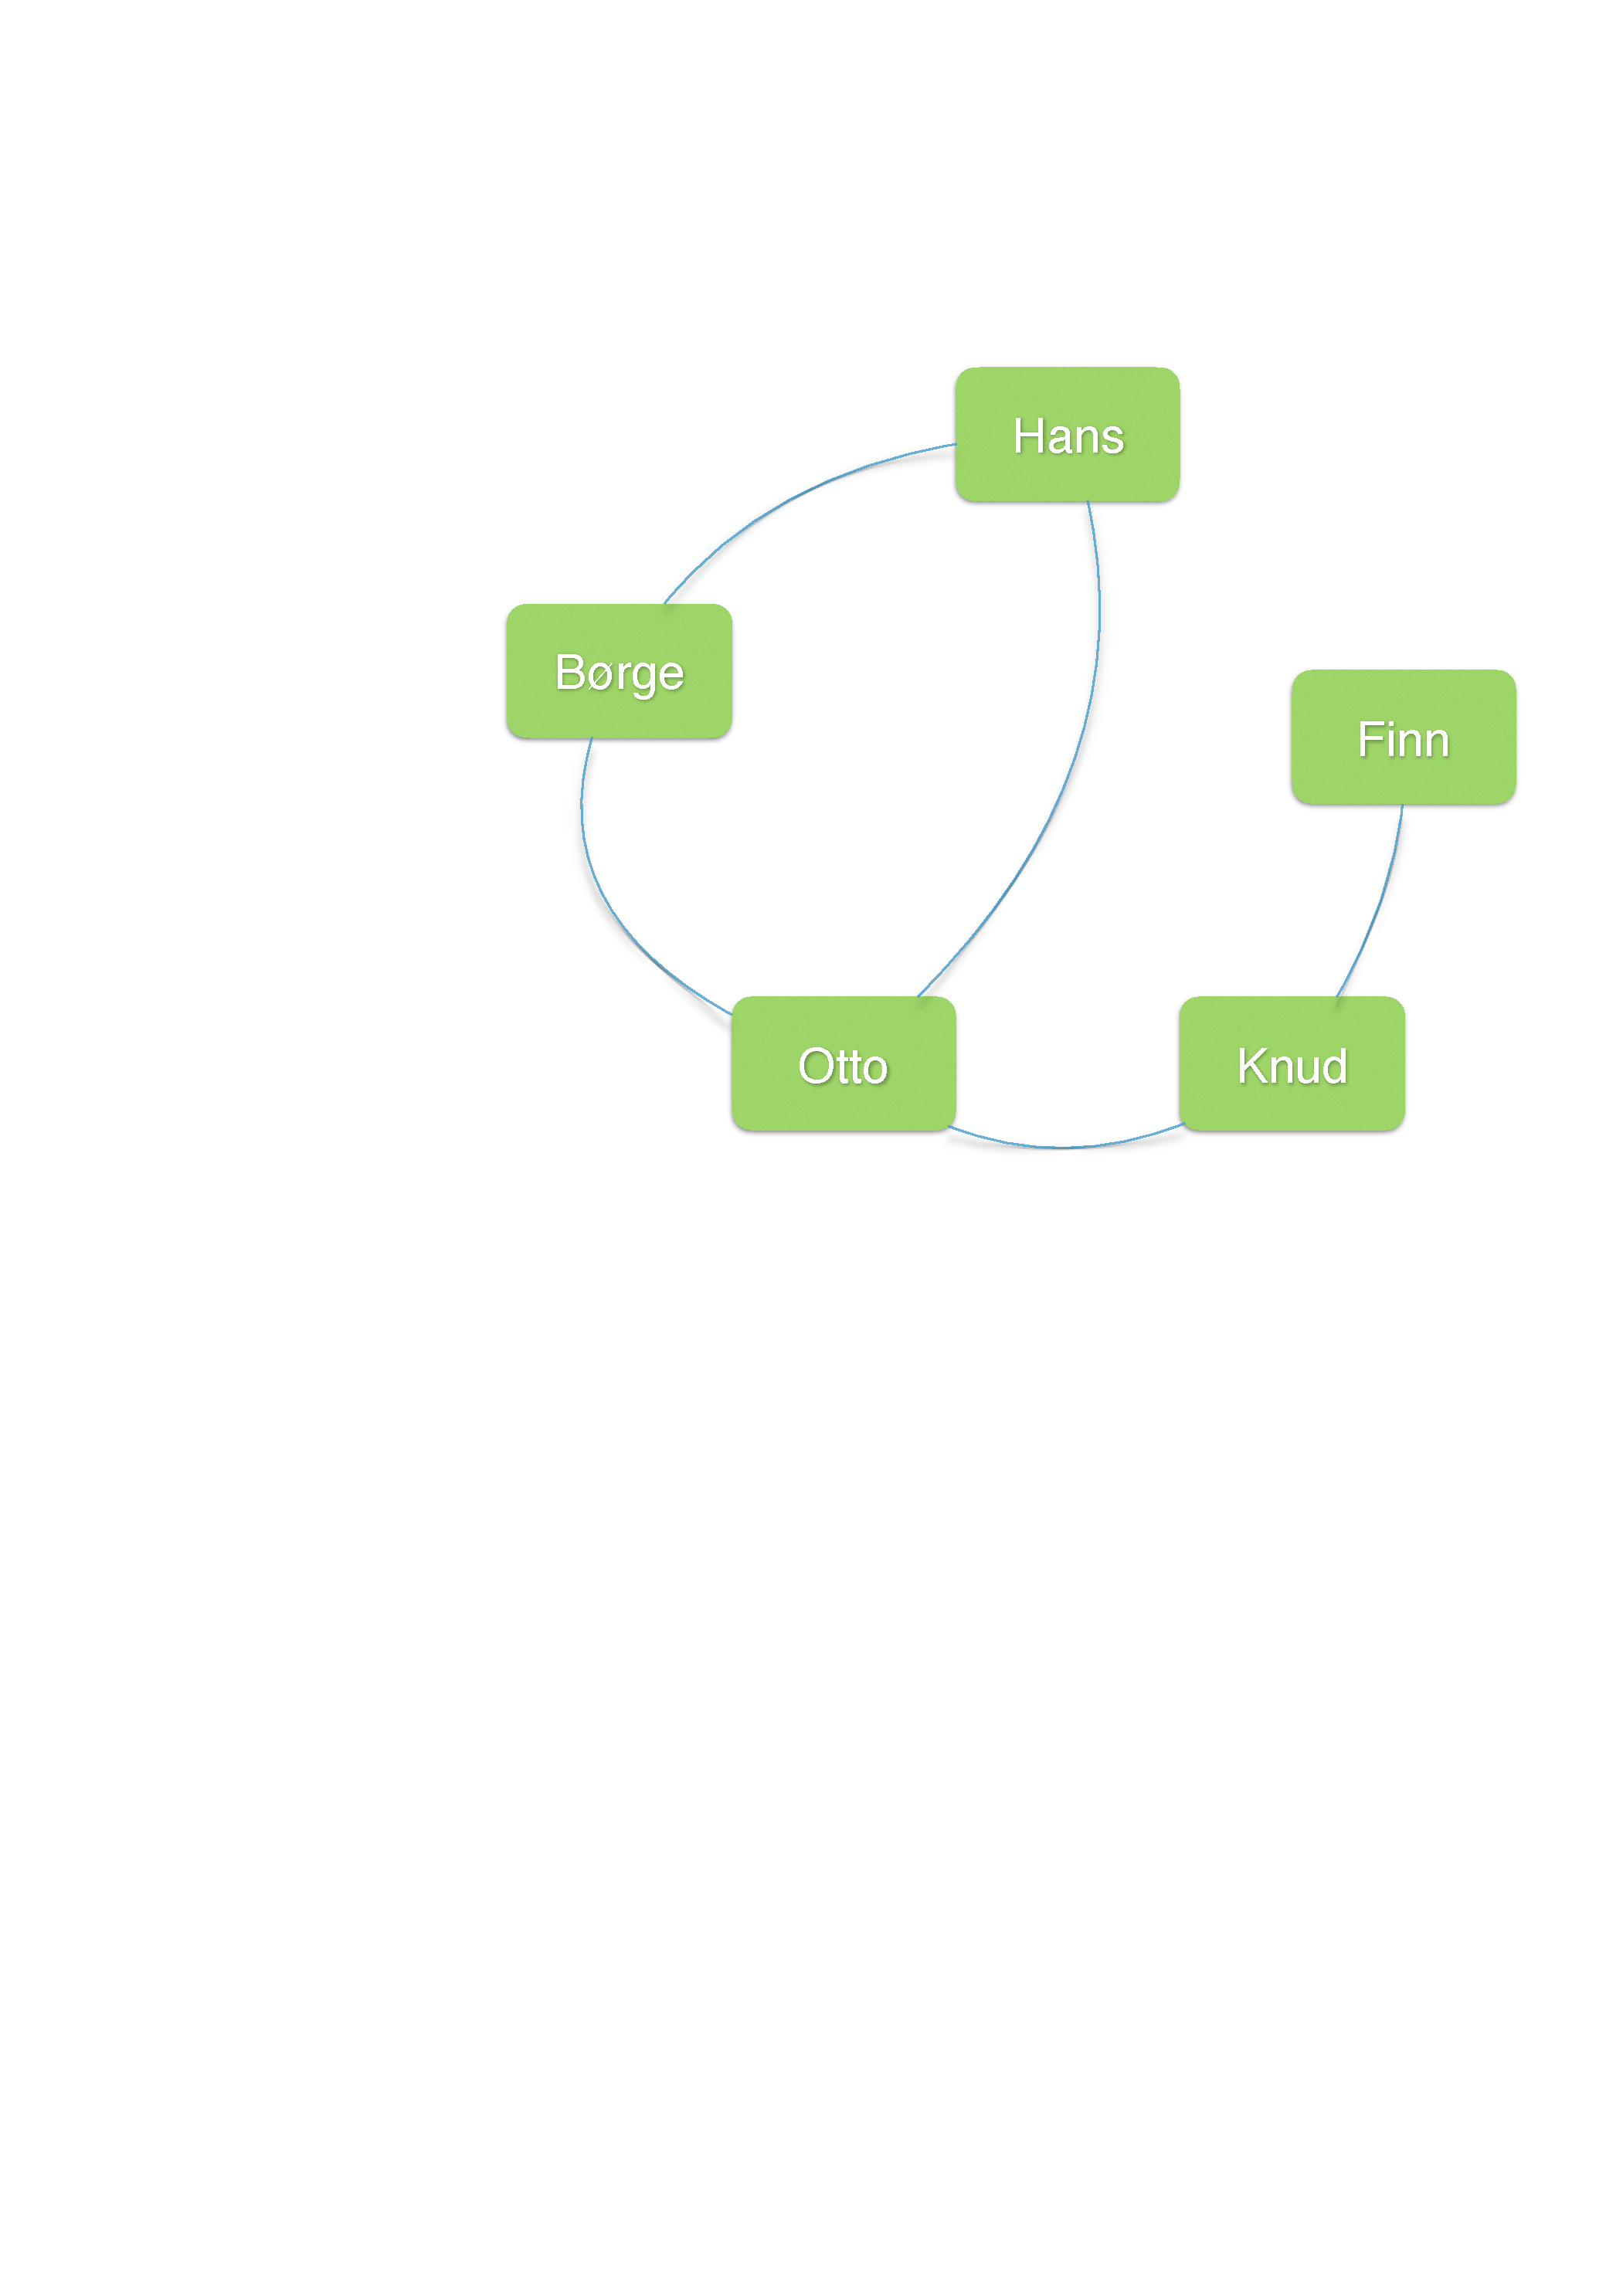
\includegraphics[width=0.4\textwidth]{example}
    \caption{Graph created from the given example of a social network.}
    \label{fig:example}
\end{figure}

\section*{Exercise M3}

The first thought for the algorithm determining if a set $X$ og persons are in a close friendship, is to run through all persons in $X$ and check if they are friends with every other person in $X$. This would have a runtime of $\Theta(k^2)$ with $k$ being the amount of persons in $X$. 

But we can deduce from the problem that there must be a relationship between the amount of persons $k$ and the amount of edges/friendship relations in $V$ (which we will call $m$). The reason for this, is the fact that a graph for a close friendship will have all nodes connected to all other nodes. This means that $m$ will have a value of 
\begin{equation*}
    m = \frac{k(k-1)}{2}
\end{equation*}

This relation is similar to triangle numbers with $k$ shifted by one. This similarity come from the fact, that for every node added to the graph, edges must be drawn to every node already existing in the graph. This means, that the algorithm only has to check how many nodes $k$ and edges $m$ are in the system. If $k$ and $m$ fulfill the relation defined above, $X$ is a close friendship. (If an edge is from a node to itself it is ignored.)

The time complexity for this algorithm is then $\Theta(k + m)$ if the quantities are not available in the data structure already, e.g. if the data structure is independent objects for each node. Alternatively if all nodes are kept in an array of nodes, and all edges are kept in an array of tuples of nodes, their lengths/sizes can be read directly (as if it was an ArrayList in java). This makes the algorithm work in constant time with time complexity $\Theta(1)$.

\section*{Exercise M4}

For Hans in the social network, there exist 3 people who are 2-friends with Hans. The nodes possible to reach using a maximum of 2 edges from Hans are: Børge, Otto and Knud.

\section*{Exercise M5}

Since $t$-friends are all nodes reachable within a limited amount of edges, we can modify the BFS searching algorithm to do this.

One way to do this is to store an array of arrays. The algoritm finds all nodes reachable using only one edge from $p$. If the node is not already in the encountered (i.e. marked as in BFS), it is stored in the an array in the array of arrays. The next iteration is to find all nodes reachable using only one edge from all the nodes in the array of nodes found in the previous iteration. These nodes are then stored in a new array in the array of arrays. This iteration happens $t$ times.

After the array of arrays is constructed, all arrays are concatenated, and the resulting array is all nodes that are $t$-friends with $p$. Just like BFS, this inspects all edges from all reached nodes, giving a worst case time complexity of O$(k + m)$ with $m$ being the amount of edges in the social network, as explained in Exercise M3. A data structure for this algorithm could be the objects for all nodes with pointers to all nodes it has an edge to. 

Another way to do this, is to have the data structure as an adjacency list, and starting with $p$ add all the neighbours of $p$ in the list and add them to a hashmap. Next iteration is to add all neighbours for the elements in the hashmap to the hashmap. This is done $t$ times, leaving all the $t$-friends of $p$ in the hashmap. By using a hashmap all duplicates get overwritten automatically. The time complexity of this algorithm is $t\cdot \text{deg}(t)$. In worst case scenario $t = k$ and $\text{deg}(p_i)=m$ for $1 \leq i \leq k$, meaning that the time complexity is O$(km)$. From Exercise M3 we have the relation between $k$ and $m$ since this is a close friendship: $km = k\cdot k(k-1)/2 = $ O$(k^3)$. 

The first algorithm is used, giving a time complexity of O$(k+m)$ using a set of node objects.

\end{document}